\documentclass[twoside]{book}

% Packages required by doxygen
\usepackage{fixltx2e}
\usepackage{calc}
\usepackage{doxygen}
\usepackage[export]{adjustbox} % also loads graphicx
\usepackage{graphicx}
\usepackage[utf8]{inputenc}
\usepackage{makeidx}
\usepackage{multicol}
\usepackage{multirow}
\PassOptionsToPackage{warn}{textcomp}
\usepackage{textcomp}
\usepackage[nointegrals]{wasysym}
\usepackage[table]{xcolor}

% Font selection
\usepackage[T1]{fontenc}
\usepackage[scaled=.90]{helvet}
\usepackage{courier}
\usepackage{amssymb}
\usepackage{sectsty}
\renewcommand{\familydefault}{\sfdefault}
\allsectionsfont{%
  \fontseries{bc}\selectfont%
  \color{darkgray}%
}
\renewcommand{\DoxyLabelFont}{%
  \fontseries{bc}\selectfont%
  \color{darkgray}%
}
\newcommand{\+}{\discretionary{\mbox{\scriptsize$\hookleftarrow$}}{}{}}

% Page & text layout
\usepackage{geometry}
\geometry{%
  a4paper,%
  top=2.5cm,%
  bottom=2.5cm,%
  left=2.5cm,%
  right=2.5cm%
}
\tolerance=750
\hfuzz=15pt
\hbadness=750
\setlength{\emergencystretch}{15pt}
\setlength{\parindent}{0cm}
\setlength{\parskip}{0.2cm}
\makeatletter
\renewcommand{\paragraph}{%
  \@startsection{paragraph}{4}{0ex}{-1.0ex}{1.0ex}{%
    \normalfont\normalsize\bfseries\SS@parafont%
  }%
}
\renewcommand{\subparagraph}{%
  \@startsection{subparagraph}{5}{0ex}{-1.0ex}{1.0ex}{%
    \normalfont\normalsize\bfseries\SS@subparafont%
  }%
}
\makeatother

% Headers & footers
\usepackage{fancyhdr}
\pagestyle{fancyplain}
\fancyhead[LE]{\fancyplain{}{\bfseries\thepage}}
\fancyhead[CE]{\fancyplain{}{}}
\fancyhead[RE]{\fancyplain{}{\bfseries\leftmark}}
\fancyhead[LO]{\fancyplain{}{\bfseries\rightmark}}
\fancyhead[CO]{\fancyplain{}{}}
\fancyhead[RO]{\fancyplain{}{\bfseries\thepage}}
\fancyfoot[LE]{\fancyplain{}{}}
\fancyfoot[CE]{\fancyplain{}{}}
\fancyfoot[RE]{\fancyplain{}{\bfseries\scriptsize Generated on Tue Mar 3 2015 15\+:04\+:21 for Task Manager by Doxygen }}
\fancyfoot[LO]{\fancyplain{}{\bfseries\scriptsize Generated on Tue Mar 3 2015 15\+:04\+:21 for Task Manager by Doxygen }}
\fancyfoot[CO]{\fancyplain{}{}}
\fancyfoot[RO]{\fancyplain{}{}}
\renewcommand{\footrulewidth}{0.4pt}
\renewcommand{\chaptermark}[1]{%
  \markboth{#1}{}%
}
\renewcommand{\sectionmark}[1]{%
  \markright{\thesection\ #1}%
}

% Indices & bibliography
\usepackage{natbib}
\usepackage[titles]{tocloft}
\setcounter{tocdepth}{3}
\setcounter{secnumdepth}{5}
\makeindex

% Hyperlinks (required, but should be loaded last)
\usepackage{ifpdf}
\ifpdf
  \usepackage[pdftex,pagebackref=true]{hyperref}
\else
  \usepackage[ps2pdf,pagebackref=true]{hyperref}
\fi
\hypersetup{%
  colorlinks=true,%
  linkcolor=blue,%
  citecolor=blue,%
  unicode%
}

% Custom commands
\newcommand{\clearemptydoublepage}{%
  \newpage{\pagestyle{empty}\cleardoublepage}%
}


%===== C O N T E N T S =====

\begin{document}

% Titlepage & ToC
\hypersetup{pageanchor=false,
             bookmarks=true,
             bookmarksnumbered=true,
             pdfencoding=unicode
            }
\pagenumbering{roman}
\begin{titlepage}
\vspace*{7cm}
\begin{center}%
{\Large Task Manager \\[1ex]\large 1.\+0 }\\
\vspace*{1cm}
{\large Generated by Doxygen 1.8.9.1}\\
\vspace*{0.5cm}
{\small Tue Mar 3 2015 15:04:21}\\
\end{center}
\end{titlepage}
\clearemptydoublepage
\tableofcontents
\clearemptydoublepage
\pagenumbering{arabic}
\hypersetup{pageanchor=true}

%--- Begin generated contents ---
\chapter{Namespace Index}
\section{Packages}
Here are the packages with brief descriptions (if available)\+:\begin{DoxyCompactList}
\item\contentsline{section}{\hyperlink{namespace_windows_forms_application1}{Windows\+Forms\+Application1} }{\pageref{namespace_windows_forms_application1}}{}
\item\contentsline{section}{\hyperlink{namespace_windows_forms_application1_1_1_controllers}{Windows\+Forms\+Application1.\+Controllers} }{\pageref{namespace_windows_forms_application1_1_1_controllers}}{}
\item\contentsline{section}{\hyperlink{namespace_windows_forms_application1_1_1_models}{Windows\+Forms\+Application1.\+Models} }{\pageref{namespace_windows_forms_application1_1_1_models}}{}
\item\contentsline{section}{\hyperlink{namespace_windows_forms_application1_1_1_properties}{Windows\+Forms\+Application1.\+Properties} }{\pageref{namespace_windows_forms_application1_1_1_properties}}{}
\end{DoxyCompactList}

\chapter{Hierarchical Index}
\section{Class Hierarchy}
This inheritance list is sorted roughly, but not completely, alphabetically\+:\begin{DoxyCompactList}
\item \contentsline{section}{Windows\+Forms\+Application1.\+Models.\+cpu\+Monitor}{\pageref{class_windows_forms_application1_1_1_models_1_1cpu_monitor}}{}
\item \contentsline{section}{Windows\+Forms\+Application1.\+Models.\+disk\+Monitor}{\pageref{class_windows_forms_application1_1_1_models_1_1disk_monitor}}{}
\item Form\begin{DoxyCompactList}
\item \contentsline{section}{Windows\+Forms\+Application1.\+Form1}{\pageref{class_windows_forms_application1_1_1_form1}}{}
\end{DoxyCompactList}
\item \contentsline{section}{Windows\+Forms\+Application1.\+Models.\+network\+Monitor}{\pageref{class_windows_forms_application1_1_1_models_1_1network_monitor}}{}
\item \contentsline{section}{Windows\+Forms\+Application1.\+Models.\+ram\+Monitor}{\pageref{class_windows_forms_application1_1_1_models_1_1ram_monitor}}{}
\item \contentsline{section}{Windows\+Forms\+Application1.\+Controllers.\+view\+Controller}{\pageref{class_windows_forms_application1_1_1_controllers_1_1view_controller}}{}
\end{DoxyCompactList}

\chapter{Class Index}
\section{Class List}
Here are the classes, structs, unions and interfaces with brief descriptions\+:\begin{DoxyCompactList}
\item\contentsline{section}{\hyperlink{class_windows_forms_application1_1_1_models_1_1cpu_monitor}{Windows\+Forms\+Application1.\+Models.\+cpu\+Monitor} }{\pageref{class_windows_forms_application1_1_1_models_1_1cpu_monitor}}{}
\item\contentsline{section}{\hyperlink{class_windows_forms_application1_1_1_models_1_1disk_monitor}{Windows\+Forms\+Application1.\+Models.\+disk\+Monitor} }{\pageref{class_windows_forms_application1_1_1_models_1_1disk_monitor}}{}
\item\contentsline{section}{\hyperlink{class_windows_forms_application1_1_1_form1}{Windows\+Forms\+Application1.\+Form1} }{\pageref{class_windows_forms_application1_1_1_form1}}{}
\item\contentsline{section}{\hyperlink{class_windows_forms_application1_1_1_models_1_1network_monitor}{Windows\+Forms\+Application1.\+Models.\+network\+Monitor} }{\pageref{class_windows_forms_application1_1_1_models_1_1network_monitor}}{}
\item\contentsline{section}{\hyperlink{class_windows_forms_application1_1_1_models_1_1ram_monitor}{Windows\+Forms\+Application1.\+Models.\+ram\+Monitor} }{\pageref{class_windows_forms_application1_1_1_models_1_1ram_monitor}}{}
\item\contentsline{section}{\hyperlink{class_windows_forms_application1_1_1_controllers_1_1view_controller}{Windows\+Forms\+Application1.\+Controllers.\+view\+Controller} \\*Controlador de vista \hyperlink{class_windows_forms_application1_1_1_form1}{Form1} }{\pageref{class_windows_forms_application1_1_1_controllers_1_1view_controller}}{}
\end{DoxyCompactList}

\chapter{File Index}
\section{File List}
Here is a list of all files with brief descriptions\+:\begin{DoxyCompactList}
\item\contentsline{section}{/\+Users/fides/\+Desktop/\+Windows\+Forms\+Application1/\+Windows\+Forms\+Application1/\hyperlink{_program_8cs}{Program.\+cs} }{\pageref{_program_8cs}}{}
\item\contentsline{section}{/\+Users/fides/\+Desktop/\+Windows\+Forms\+Application1/\+Windows\+Forms\+Application1/\+Controllers/\hyperlink{view_controller_8cs}{view\+Controller.\+cs} }{\pageref{view_controller_8cs}}{}
\item\contentsline{section}{/\+Users/fides/\+Desktop/\+Windows\+Forms\+Application1/\+Windows\+Forms\+Application1/\+Models/\hyperlink{cpu_monitor_8cs}{cpu\+Monitor.\+cs} }{\pageref{cpu_monitor_8cs}}{}
\item\contentsline{section}{/\+Users/fides/\+Desktop/\+Windows\+Forms\+Application1/\+Windows\+Forms\+Application1/\+Models/\hyperlink{disk_monitor_8cs}{disk\+Monitor.\+cs} }{\pageref{disk_monitor_8cs}}{}
\item\contentsline{section}{/\+Users/fides/\+Desktop/\+Windows\+Forms\+Application1/\+Windows\+Forms\+Application1/\+Models/\hyperlink{network_monitor_8cs}{network\+Monitor.\+cs} }{\pageref{network_monitor_8cs}}{}
\item\contentsline{section}{/\+Users/fides/\+Desktop/\+Windows\+Forms\+Application1/\+Windows\+Forms\+Application1/\+Models/\hyperlink{ram_monitor_8cs}{ram\+Monitor.\+cs} }{\pageref{ram_monitor_8cs}}{}
\item\contentsline{section}{/\+Users/fides/\+Desktop/\+Windows\+Forms\+Application1/\+Windows\+Forms\+Application1/obj/\+Debug/\hyperlink{_temporary_generated_file__036_c0_b5_b-1481-4323-8_d20-8_f5_a_d_c_b23_d92_8cs}{Temporary\+Generated\+File\+\_\+036\+C0\+B5\+B-\/1481-\/4323-\/8\+D20-\/8\+F5\+A\+D\+C\+B23\+D92.\+cs} }{\pageref{_temporary_generated_file__036_c0_b5_b-1481-4323-8_d20-8_f5_a_d_c_b23_d92_8cs}}{}
\item\contentsline{section}{/\+Users/fides/\+Desktop/\+Windows\+Forms\+Application1/\+Windows\+Forms\+Application1/obj/\+Debug/\hyperlink{_temporary_generated_file__5937a670-0e60-4077-877b-f7221da3dda1_8cs}{Temporary\+Generated\+File\+\_\+5937a670-\/0e60-\/4077-\/877b-\/f7221da3dda1.\+cs} }{\pageref{_temporary_generated_file__5937a670-0e60-4077-877b-f7221da3dda1_8cs}}{}
\item\contentsline{section}{/\+Users/fides/\+Desktop/\+Windows\+Forms\+Application1/\+Windows\+Forms\+Application1/obj/\+Debug/\hyperlink{_temporary_generated_file___e7_a71_f73-0_f8_d-4_b9_b-_b56_e-8_e70_b10_b_c5_d3_8cs}{Temporary\+Generated\+File\+\_\+\+E7\+A71\+F73-\/0\+F8\+D-\/4\+B9\+B-\/\+B56\+E-\/8\+E70\+B10\+B\+C5\+D3.\+cs} }{\pageref{_temporary_generated_file___e7_a71_f73-0_f8_d-4_b9_b-_b56_e-8_e70_b10_b_c5_d3_8cs}}{}
\item\contentsline{section}{/\+Users/fides/\+Desktop/\+Windows\+Forms\+Application1/\+Windows\+Forms\+Application1/\+Properties/\hyperlink{_assembly_info_8cs}{Assembly\+Info.\+cs} }{\pageref{_assembly_info_8cs}}{}
\item\contentsline{section}{/\+Users/fides/\+Desktop/\+Windows\+Forms\+Application1/\+Windows\+Forms\+Application1/\+Properties/\hyperlink{_resources_8_designer_8cs}{Resources.\+Designer.\+cs} }{\pageref{_resources_8_designer_8cs}}{}
\item\contentsline{section}{/\+Users/fides/\+Desktop/\+Windows\+Forms\+Application1/\+Windows\+Forms\+Application1/\+Properties/\hyperlink{_settings_8_designer_8cs}{Settings.\+Designer.\+cs} }{\pageref{_settings_8_designer_8cs}}{}
\item\contentsline{section}{/\+Users/fides/\+Desktop/\+Windows\+Forms\+Application1/\+Windows\+Forms\+Application1/\+Views/\hyperlink{view_8cs}{view.\+cs} }{\pageref{view_8cs}}{}
\item\contentsline{section}{/\+Users/fides/\+Desktop/\+Windows\+Forms\+Application1/\+Windows\+Forms\+Application1/\+Views/\hyperlink{view_8_designer_8cs}{view.\+Designer.\+cs} }{\pageref{view_8_designer_8cs}}{}
\end{DoxyCompactList}

\chapter{Namespace Documentation}
\hypertarget{namespace_windows_forms_application1}{}\section{Package Windows\+Forms\+Application1}
\label{namespace_windows_forms_application1}\index{Windows\+Forms\+Application1@{Windows\+Forms\+Application1}}
\subsection*{Namespaces}
\begin{DoxyCompactItemize}
\item 
package \hyperlink{namespace_windows_forms_application1_1_1_controllers}{Controllers}
\item 
package \hyperlink{namespace_windows_forms_application1_1_1_models}{Models}
\item 
package \hyperlink{namespace_windows_forms_application1_1_1_properties}{Properties}
\end{DoxyCompactItemize}
\subsection*{Classes}
\begin{DoxyCompactItemize}
\item 
class \hyperlink{class_windows_forms_application1_1_1_form1}{Form1}
\item 
class {\bfseries Program}
\end{DoxyCompactItemize}

\hypertarget{namespace_windows_forms_application1_1_1_controllers}{}\section{Package Windows\+Forms\+Application1.\+Controllers}
\label{namespace_windows_forms_application1_1_1_controllers}\index{Windows\+Forms\+Application1.\+Controllers@{Windows\+Forms\+Application1.\+Controllers}}
\subsection*{Classes}
\begin{DoxyCompactItemize}
\item 
class \hyperlink{class_windows_forms_application1_1_1_controllers_1_1view_controller}{view\+Controller}
\begin{DoxyCompactList}\small\item\em Controlador de vista \hyperlink{class_windows_forms_application1_1_1_form1}{Form1} \end{DoxyCompactList}\end{DoxyCompactItemize}

\hypertarget{namespace_windows_forms_application1_1_1_models}{}\section{Package Windows\+Forms\+Application1.\+Models}
\label{namespace_windows_forms_application1_1_1_models}\index{Windows\+Forms\+Application1.\+Models@{Windows\+Forms\+Application1.\+Models}}
\subsection*{Classes}
\begin{DoxyCompactItemize}
\item 
class \hyperlink{class_windows_forms_application1_1_1_models_1_1cpu_monitor}{cpu\+Monitor}
\item 
class \hyperlink{class_windows_forms_application1_1_1_models_1_1disk_monitor}{disk\+Monitor}
\item 
class \hyperlink{class_windows_forms_application1_1_1_models_1_1network_monitor}{network\+Monitor}
\item 
class \hyperlink{class_windows_forms_application1_1_1_models_1_1ram_monitor}{ram\+Monitor}
\end{DoxyCompactItemize}

\hypertarget{namespace_windows_forms_application1_1_1_properties}{}\section{Package Windows\+Forms\+Application1.\+Properties}
\label{namespace_windows_forms_application1_1_1_properties}\index{Windows\+Forms\+Application1.\+Properties@{Windows\+Forms\+Application1.\+Properties}}
\subsection*{Classes}
\begin{DoxyCompactItemize}
\item 
class {\bfseries Resources}
\begin{DoxyCompactList}\small\item\em A strongly-\/typed resource class, for looking up localized strings, etc. \end{DoxyCompactList}\item 
class {\bfseries Settings}
\end{DoxyCompactItemize}

\chapter{Class Documentation}
\hypertarget{class_windows_forms_application1_1_1_models_1_1cpu_monitor}{}\section{Windows\+Forms\+Application1.\+Models.\+cpu\+Monitor Class Reference}
\label{class_windows_forms_application1_1_1_models_1_1cpu_monitor}\index{Windows\+Forms\+Application1.\+Models.\+cpu\+Monitor@{Windows\+Forms\+Application1.\+Models.\+cpu\+Monitor}}
\subsection*{Public Member Functions}
\begin{DoxyCompactItemize}
\item 
\hyperlink{class_windows_forms_application1_1_1_models_1_1cpu_monitor_aa93e334b10d2ecf00c55e266846467e2}{cpu\+Monitor} (int interval\+Time\+Out, \hyperlink{class_windows_forms_application1_1_1_form1}{Form1} cte)
\begin{DoxyCompactList}\small\item\em Constructor. \end{DoxyCompactList}\item 
void \hyperlink{class_windows_forms_application1_1_1_models_1_1cpu_monitor_ab10f241a0b2ee431cb44daf3a0f8e972}{Start} ()
\begin{DoxyCompactList}\small\item\em metodo para iniciar el treath crea el nuevo thread y asigna metodo de ejeccucion (run) \end{DoxyCompactList}\item 
Double \hyperlink{class_windows_forms_application1_1_1_models_1_1cpu_monitor_ab9b7d5ae64eac03b98d128bb1c42e900}{Get\+Processor\+Data} ()
\begin{DoxyCompactList}\small\item\em wrapper para simplicidad de funcion Get\+Counter\+Value \end{DoxyCompactList}\end{DoxyCompactItemize}


\subsection{Detailed Description}


Definition at line 11 of file cpu\+Monitor.\+cs.



\subsection{Constructor \& Destructor Documentation}
\hypertarget{class_windows_forms_application1_1_1_models_1_1cpu_monitor_aa93e334b10d2ecf00c55e266846467e2}{}\index{Windows\+Forms\+Application1\+::\+Models\+::cpu\+Monitor@{Windows\+Forms\+Application1\+::\+Models\+::cpu\+Monitor}!cpu\+Monitor@{cpu\+Monitor}}
\index{cpu\+Monitor@{cpu\+Monitor}!Windows\+Forms\+Application1\+::\+Models\+::cpu\+Monitor@{Windows\+Forms\+Application1\+::\+Models\+::cpu\+Monitor}}
\subsubsection[{cpu\+Monitor}]{\setlength{\rightskip}{0pt plus 5cm}Windows\+Forms\+Application1.\+Models.\+cpu\+Monitor.\+cpu\+Monitor (
\begin{DoxyParamCaption}
\item[{int}]{interval\+Time\+Out, }
\item[{{\bf Form1}}]{cte}
\end{DoxyParamCaption}
)}\label{class_windows_forms_application1_1_1_models_1_1cpu_monitor_aa93e334b10d2ecf00c55e266846467e2}


Constructor. 


\begin{DoxyParams}{Parameters}
{\em interval\+Time\+Out} & tiempo de sleep\\
\hline
{\em cte} & referencia al contexto de U\+X\\
\hline
\end{DoxyParams}


Definition at line 38 of file cpu\+Monitor.\+cs.



\subsection{Member Function Documentation}
\hypertarget{class_windows_forms_application1_1_1_models_1_1cpu_monitor_ab9b7d5ae64eac03b98d128bb1c42e900}{}\index{Windows\+Forms\+Application1\+::\+Models\+::cpu\+Monitor@{Windows\+Forms\+Application1\+::\+Models\+::cpu\+Monitor}!Get\+Processor\+Data@{Get\+Processor\+Data}}
\index{Get\+Processor\+Data@{Get\+Processor\+Data}!Windows\+Forms\+Application1\+::\+Models\+::cpu\+Monitor@{Windows\+Forms\+Application1\+::\+Models\+::cpu\+Monitor}}
\subsubsection[{Get\+Processor\+Data}]{\setlength{\rightskip}{0pt plus 5cm}Double Windows\+Forms\+Application1.\+Models.\+cpu\+Monitor.\+Get\+Processor\+Data (
\begin{DoxyParamCaption}
{}
\end{DoxyParamCaption}
)}\label{class_windows_forms_application1_1_1_models_1_1cpu_monitor_ab9b7d5ae64eac03b98d128bb1c42e900}


wrapper para simplicidad de funcion Get\+Counter\+Value 

\begin{DoxyReturn}{Returns}
Double con valor del total del procesador
\end{DoxyReturn}


Definition at line 85 of file cpu\+Monitor.\+cs.

\hypertarget{class_windows_forms_application1_1_1_models_1_1cpu_monitor_ab10f241a0b2ee431cb44daf3a0f8e972}{}\index{Windows\+Forms\+Application1\+::\+Models\+::cpu\+Monitor@{Windows\+Forms\+Application1\+::\+Models\+::cpu\+Monitor}!Start@{Start}}
\index{Start@{Start}!Windows\+Forms\+Application1\+::\+Models\+::cpu\+Monitor@{Windows\+Forms\+Application1\+::\+Models\+::cpu\+Monitor}}
\subsubsection[{Start}]{\setlength{\rightskip}{0pt plus 5cm}void Windows\+Forms\+Application1.\+Models.\+cpu\+Monitor.\+Start (
\begin{DoxyParamCaption}
{}
\end{DoxyParamCaption}
)}\label{class_windows_forms_application1_1_1_models_1_1cpu_monitor_ab10f241a0b2ee431cb44daf3a0f8e972}


metodo para iniciar el treath crea el nuevo thread y asigna metodo de ejeccucion (run) 



Definition at line 48 of file cpu\+Monitor.\+cs.



The documentation for this class was generated from the following file\+:\begin{DoxyCompactItemize}
\item 
/\+Users/fides/\+Desktop/\+Windows\+Forms\+Application1/\+Windows\+Forms\+Application1/\+Models/\hyperlink{cpu_monitor_8cs}{cpu\+Monitor.\+cs}\end{DoxyCompactItemize}

\hypertarget{class_windows_forms_application1_1_1_models_1_1disk_monitor}{}\section{Windows\+Forms\+Application1.\+Models.\+disk\+Monitor Class Reference}
\label{class_windows_forms_application1_1_1_models_1_1disk_monitor}\index{Windows\+Forms\+Application1.\+Models.\+disk\+Monitor@{Windows\+Forms\+Application1.\+Models.\+disk\+Monitor}}
\subsection*{Public Types}
\begin{DoxyCompactItemize}
\item 
enum \hyperlink{class_windows_forms_application1_1_1_models_1_1disk_monitor_a5e72e797fa7e0095f80d5069b11ae0ec}{tipo\+Operacion\+Disco} \{ \hyperlink{class_windows_forms_application1_1_1_models_1_1disk_monitor_a5e72e797fa7e0095f80d5069b11ae0eca38ca42a40fd96052406452e916cc22ad}{tipo\+Operacion\+Disco.\+Read\+And\+Write}, 
\hyperlink{class_windows_forms_application1_1_1_models_1_1disk_monitor_a5e72e797fa7e0095f80d5069b11ae0eca7a1a5f3e79fdc91edf2f5ead9d66abb4}{tipo\+Operacion\+Disco.\+Read}, 
\hyperlink{class_windows_forms_application1_1_1_models_1_1disk_monitor_a5e72e797fa7e0095f80d5069b11ae0eca1129c0e4d43f2d121652a7302712cff6}{tipo\+Operacion\+Disco.\+Write}
 \}
\begin{DoxyCompactList}\small\item\em diccionario para seleccionar tipo de acceso a medir. \end{DoxyCompactList}\end{DoxyCompactItemize}
\subsection*{Public Member Functions}
\begin{DoxyCompactItemize}
\item 
\hyperlink{class_windows_forms_application1_1_1_models_1_1disk_monitor_a1adc13f29078356113f2688eef9c1d70}{disk\+Monitor} (int interval\+Time\+Out, \hyperlink{class_windows_forms_application1_1_1_form1}{Form1} cte)
\begin{DoxyCompactList}\small\item\em Construcctor de la clase \end{DoxyCompactList}\item 
void \hyperlink{class_windows_forms_application1_1_1_models_1_1disk_monitor_aea00f90a1d1f844635454060c76133a0}{Start} ()
\begin{DoxyCompactList}\small\item\em crea un thread y lo inicia \end{DoxyCompactList}\item 
double \hyperlink{class_windows_forms_application1_1_1_models_1_1disk_monitor_a3d5bf64d33553c41813a96769b898503}{Get\+Disk\+Data} (\hyperlink{class_windows_forms_application1_1_1_models_1_1disk_monitor_a5e72e797fa7e0095f80d5069b11ae0ec}{tipo\+Operacion\+Disco} tipo\+Acceso)
\begin{DoxyCompactList}\small\item\em funcion para obtener la velodicidad del disco, funciona para lectura, escritura, y lectura/escritura. \end{DoxyCompactList}\end{DoxyCompactItemize}


\subsection{Detailed Description}


Definition at line 11 of file disk\+Monitor.\+cs.



\subsection{Member Enumeration Documentation}
\hypertarget{class_windows_forms_application1_1_1_models_1_1disk_monitor_a5e72e797fa7e0095f80d5069b11ae0ec}{}\index{Windows\+Forms\+Application1\+::\+Models\+::disk\+Monitor@{Windows\+Forms\+Application1\+::\+Models\+::disk\+Monitor}!tipo\+Operacion\+Disco@{tipo\+Operacion\+Disco}}
\index{tipo\+Operacion\+Disco@{tipo\+Operacion\+Disco}!Windows\+Forms\+Application1\+::\+Models\+::disk\+Monitor@{Windows\+Forms\+Application1\+::\+Models\+::disk\+Monitor}}
\subsubsection[{tipo\+Operacion\+Disco}]{\setlength{\rightskip}{0pt plus 5cm}enum {\bf Windows\+Forms\+Application1.\+Models.\+disk\+Monitor.\+tipo\+Operacion\+Disco}}\label{class_windows_forms_application1_1_1_models_1_1disk_monitor_a5e72e797fa7e0095f80d5069b11ae0ec}


diccionario para seleccionar tipo de acceso a medir. 

\begin{Desc}
\item[Enumerator]\par
\begin{description}
\index{Read\+And\+Write@{Read\+And\+Write}!Windows\+Forms\+Application1\+::\+Models\+::disk\+Monitor@{Windows\+Forms\+Application1\+::\+Models\+::disk\+Monitor}}\index{Windows\+Forms\+Application1\+::\+Models\+::disk\+Monitor@{Windows\+Forms\+Application1\+::\+Models\+::disk\+Monitor}!Read\+And\+Write@{Read\+And\+Write}}\item[{\em 
\hypertarget{class_windows_forms_application1_1_1_models_1_1disk_monitor_a5e72e797fa7e0095f80d5069b11ae0eca38ca42a40fd96052406452e916cc22ad}{}Read\+And\+Write\label{class_windows_forms_application1_1_1_models_1_1disk_monitor_a5e72e797fa7e0095f80d5069b11ae0eca38ca42a40fd96052406452e916cc22ad}
}]\index{Read@{Read}!Windows\+Forms\+Application1\+::\+Models\+::disk\+Monitor@{Windows\+Forms\+Application1\+::\+Models\+::disk\+Monitor}}\index{Windows\+Forms\+Application1\+::\+Models\+::disk\+Monitor@{Windows\+Forms\+Application1\+::\+Models\+::disk\+Monitor}!Read@{Read}}\item[{\em 
\hypertarget{class_windows_forms_application1_1_1_models_1_1disk_monitor_a5e72e797fa7e0095f80d5069b11ae0eca7a1a5f3e79fdc91edf2f5ead9d66abb4}{}Read\label{class_windows_forms_application1_1_1_models_1_1disk_monitor_a5e72e797fa7e0095f80d5069b11ae0eca7a1a5f3e79fdc91edf2f5ead9d66abb4}
}]\index{Write@{Write}!Windows\+Forms\+Application1\+::\+Models\+::disk\+Monitor@{Windows\+Forms\+Application1\+::\+Models\+::disk\+Monitor}}\index{Windows\+Forms\+Application1\+::\+Models\+::disk\+Monitor@{Windows\+Forms\+Application1\+::\+Models\+::disk\+Monitor}!Write@{Write}}\item[{\em 
\hypertarget{class_windows_forms_application1_1_1_models_1_1disk_monitor_a5e72e797fa7e0095f80d5069b11ae0eca1129c0e4d43f2d121652a7302712cff6}{}Write\label{class_windows_forms_application1_1_1_models_1_1disk_monitor_a5e72e797fa7e0095f80d5069b11ae0eca1129c0e4d43f2d121652a7302712cff6}
}]\end{description}
\end{Desc}


Definition at line 38 of file disk\+Monitor.\+cs.



\subsection{Constructor \& Destructor Documentation}
\hypertarget{class_windows_forms_application1_1_1_models_1_1disk_monitor_a1adc13f29078356113f2688eef9c1d70}{}\index{Windows\+Forms\+Application1\+::\+Models\+::disk\+Monitor@{Windows\+Forms\+Application1\+::\+Models\+::disk\+Monitor}!disk\+Monitor@{disk\+Monitor}}
\index{disk\+Monitor@{disk\+Monitor}!Windows\+Forms\+Application1\+::\+Models\+::disk\+Monitor@{Windows\+Forms\+Application1\+::\+Models\+::disk\+Monitor}}
\subsubsection[{disk\+Monitor}]{\setlength{\rightskip}{0pt plus 5cm}Windows\+Forms\+Application1.\+Models.\+disk\+Monitor.\+disk\+Monitor (
\begin{DoxyParamCaption}
\item[{int}]{interval\+Time\+Out, }
\item[{{\bf Form1}}]{cte}
\end{DoxyParamCaption}
)}\label{class_windows_forms_application1_1_1_models_1_1disk_monitor_a1adc13f29078356113f2688eef9c1d70}


Construcctor de la clase 


\begin{DoxyParams}{Parameters}
{\em interval\+Time\+Out} & tiempo para sleep\\
\hline
{\em cte} & contexto de interfaz\\
\hline
\end{DoxyParams}


Definition at line 54 of file disk\+Monitor.\+cs.



\subsection{Member Function Documentation}
\hypertarget{class_windows_forms_application1_1_1_models_1_1disk_monitor_a3d5bf64d33553c41813a96769b898503}{}\index{Windows\+Forms\+Application1\+::\+Models\+::disk\+Monitor@{Windows\+Forms\+Application1\+::\+Models\+::disk\+Monitor}!Get\+Disk\+Data@{Get\+Disk\+Data}}
\index{Get\+Disk\+Data@{Get\+Disk\+Data}!Windows\+Forms\+Application1\+::\+Models\+::disk\+Monitor@{Windows\+Forms\+Application1\+::\+Models\+::disk\+Monitor}}
\subsubsection[{Get\+Disk\+Data}]{\setlength{\rightskip}{0pt plus 5cm}double Windows\+Forms\+Application1.\+Models.\+disk\+Monitor.\+Get\+Disk\+Data (
\begin{DoxyParamCaption}
\item[{{\bf tipo\+Operacion\+Disco}}]{tipo\+Acceso}
\end{DoxyParamCaption}
)}\label{class_windows_forms_application1_1_1_models_1_1disk_monitor_a3d5bf64d33553c41813a96769b898503}


funcion para obtener la velodicidad del disco, funciona para lectura, escritura, y lectura/escritura. 


\begin{DoxyParams}{Parameters}
{\em tipo\+Acceso} & indica tipo de acceso.\\
\hline
\end{DoxyParams}
\begin{DoxyReturn}{Returns}
double con informacion solicitada en Bytes/sec
\end{DoxyReturn}


Definition at line 104 of file disk\+Monitor.\+cs.

\hypertarget{class_windows_forms_application1_1_1_models_1_1disk_monitor_aea00f90a1d1f844635454060c76133a0}{}\index{Windows\+Forms\+Application1\+::\+Models\+::disk\+Monitor@{Windows\+Forms\+Application1\+::\+Models\+::disk\+Monitor}!Start@{Start}}
\index{Start@{Start}!Windows\+Forms\+Application1\+::\+Models\+::disk\+Monitor@{Windows\+Forms\+Application1\+::\+Models\+::disk\+Monitor}}
\subsubsection[{Start}]{\setlength{\rightskip}{0pt plus 5cm}void Windows\+Forms\+Application1.\+Models.\+disk\+Monitor.\+Start (
\begin{DoxyParamCaption}
{}
\end{DoxyParamCaption}
)}\label{class_windows_forms_application1_1_1_models_1_1disk_monitor_aea00f90a1d1f844635454060c76133a0}


crea un thread y lo inicia 



Definition at line 63 of file disk\+Monitor.\+cs.



The documentation for this class was generated from the following file\+:\begin{DoxyCompactItemize}
\item 
/\+Users/fides/\+Desktop/\+Windows\+Forms\+Application1/\+Windows\+Forms\+Application1/\+Models/\hyperlink{disk_monitor_8cs}{disk\+Monitor.\+cs}\end{DoxyCompactItemize}

\hypertarget{class_windows_forms_application1_1_1_form1}{}\section{Windows\+Forms\+Application1.\+Form1 Class Reference}
\label{class_windows_forms_application1_1_1_form1}\index{Windows\+Forms\+Application1.\+Form1@{Windows\+Forms\+Application1.\+Form1}}
Inheritance diagram for Windows\+Forms\+Application1.\+Form1\+:\begin{figure}[H]
\begin{center}
\leavevmode
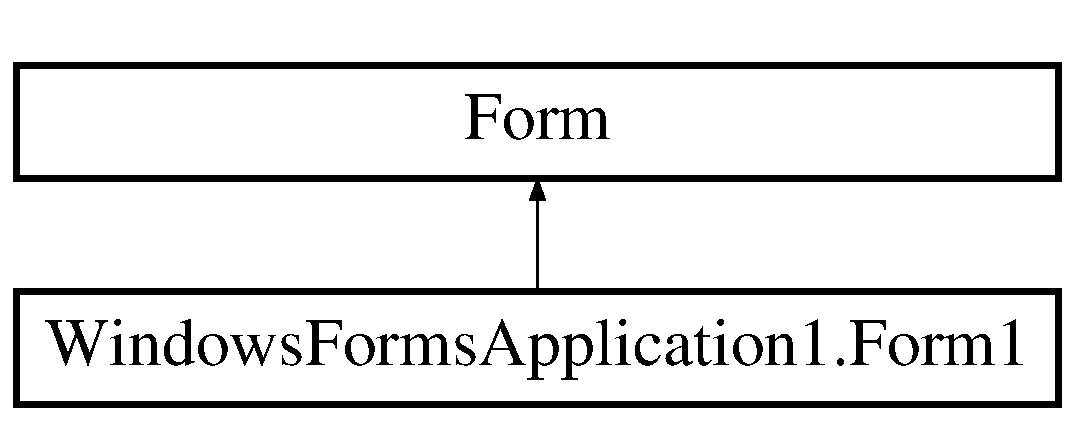
\includegraphics[height=2.000000cm]{class_windows_forms_application1_1_1_form1}
\end{center}
\end{figure}
\subsection*{Public Member Functions}
\begin{DoxyCompactItemize}
\item 
\hyperlink{class_windows_forms_application1_1_1_form1_a69c9068cd58521646d5e961a8b88a020}{Form1} ()
\begin{DoxyCompactList}\small\item\em Constructor de la clase de vista inicializa componentes y controlador de vista (M\+V\+C) //llama funcion para el estilo de las graficas \end{DoxyCompactList}\item 
void \hyperlink{class_windows_forms_application1_1_1_form1_a4fda0d42358d44b8d3912a8e4d20e914}{Set\+Ram\+Virtual} (Double total, Double usada, Double porcentaje)
\begin{DoxyCompactList}\small\item\em metodo auxiliar para actualizar interfaz de usuario. verifica si fue invocada por otro thread y de ser asi obtiene la firma del thread de de U\+X y se invoca a si mismo por medio del delegate actualiza grafica y labels necesarios \end{DoxyCompactList}\item 
void \hyperlink{class_windows_forms_application1_1_1_form1_afac9f5fe44220f30b2e8ec3750abd874}{Set\+Ram\+Fisica} (Double total, Double usada, Double porcentaje)
\begin{DoxyCompactList}\small\item\em metodo auxiliar para actualizar interfaz de usuario. verifica si fue invocada por otro thread y de ser asi obtiene la firma del thread de de U\+X y se invoca a si mismo por medio del delegate actualiza grafica y labels necesarios \end{DoxyCompactList}\end{DoxyCompactItemize}
\subsection*{Protected Member Functions}
\begin{DoxyCompactItemize}
\item 
override void \hyperlink{class_windows_forms_application1_1_1_form1_a634a80ac7348fe429fa032d0edffee00}{Dispose} (bool disposing)
\begin{DoxyCompactList}\small\item\em Clean up any resources being used. \end{DoxyCompactList}\end{DoxyCompactItemize}
\subsection*{Properties}
\begin{DoxyCompactItemize}
\item 
Double \hyperlink{class_windows_forms_application1_1_1_form1_ae445eb3f9ea10205e542590e77476e47}{cpu\+Usage}\hspace{0.3cm}{\ttfamily  \mbox{[}set\mbox{]}}
\begin{DoxyCompactList}\small\item\em metodo para asignar el uso de C\+P\+U redondea el valor a dos digitos hacia arriba y utiliza un metodo auxiliar para asignarlo. \end{DoxyCompactList}\item 
Double \hyperlink{class_windows_forms_application1_1_1_form1_af1ec7463a818d88cbf71689bbd444ab8}{cpu\+Idle}\hspace{0.3cm}{\ttfamily  \mbox{[}set\mbox{]}}
\begin{DoxyCompactList}\small\item\em metodo para asignar el del C\+P\+U que no esta uso. redondea el valor a dos digitos haci a arriba y utiliza un metodo auxiliar para asignarlo. \end{DoxyCompactList}\item 
Double \hyperlink{class_windows_forms_application1_1_1_form1_a21165d5313e265bc99107b4bcb60cdad}{disk\+Write}\hspace{0.3cm}{\ttfamily  \mbox{[}set\mbox{]}}
\begin{DoxyCompactList}\small\item\em metodo para asignar la velocidad de escritrua del disco. redondea el valor a dos digitos hacia arriba y utiliza un metodo auxiliar para asignarlo. \end{DoxyCompactList}\item 
Double \hyperlink{class_windows_forms_application1_1_1_form1_a99946d55dca3d347b344e9810b15a6d2}{disk\+Reads}\hspace{0.3cm}{\ttfamily  \mbox{[}set\mbox{]}}
\begin{DoxyCompactList}\small\item\em metodo para asignar la velocidad de lectura del disco. Redondea el valor a dos digitos hacia arriba y utiliza un metodo auxiliar para asignarlo. \end{DoxyCompactList}\item 
Double \hyperlink{class_windows_forms_application1_1_1_form1_a50fa7fa857eb7587ab11e7b2c502f240}{net\+Outs}\hspace{0.3cm}{\ttfamily  \mbox{[}set\mbox{]}}
\begin{DoxyCompactList}\small\item\em Metodo para asignar la velocidad de bites enviados por red redondea el valor a dos digitos hacia arriba y utiliza un metodo auxiliar para asignarlo. \end{DoxyCompactList}\item 
Double \hyperlink{class_windows_forms_application1_1_1_form1_ad6c6884d7846134ca9a860197d7ea0b6}{net\+Ins}\hspace{0.3cm}{\ttfamily  \mbox{[}set\mbox{]}}
\begin{DoxyCompactList}\small\item\em Metodo para asignar la velocidad de bites recibidos por red redondea el valor a dos digitos hacia arriba y utiliza un metodo auxiliar para asignarlo. \end{DoxyCompactList}\end{DoxyCompactItemize}


\subsection{Detailed Description}


Definition at line 16 of file view.\+cs.



\subsection{Constructor \& Destructor Documentation}
\hypertarget{class_windows_forms_application1_1_1_form1_a69c9068cd58521646d5e961a8b88a020}{}\index{Windows\+Forms\+Application1\+::\+Form1@{Windows\+Forms\+Application1\+::\+Form1}!Form1@{Form1}}
\index{Form1@{Form1}!Windows\+Forms\+Application1\+::\+Form1@{Windows\+Forms\+Application1\+::\+Form1}}
\subsubsection[{Form1}]{\setlength{\rightskip}{0pt plus 5cm}Windows\+Forms\+Application1.\+Form1.\+Form1 (
\begin{DoxyParamCaption}
{}
\end{DoxyParamCaption}
)}\label{class_windows_forms_application1_1_1_form1_a69c9068cd58521646d5e961a8b88a020}


Constructor de la clase de vista inicializa componentes y controlador de vista (M\+V\+C) //llama funcion para el estilo de las graficas 



Definition at line 25 of file view.\+cs.



\subsection{Member Function Documentation}
\hypertarget{class_windows_forms_application1_1_1_form1_a634a80ac7348fe429fa032d0edffee00}{}\index{Windows\+Forms\+Application1\+::\+Form1@{Windows\+Forms\+Application1\+::\+Form1}!Dispose@{Dispose}}
\index{Dispose@{Dispose}!Windows\+Forms\+Application1\+::\+Form1@{Windows\+Forms\+Application1\+::\+Form1}}
\subsubsection[{Dispose}]{\setlength{\rightskip}{0pt plus 5cm}override void Windows\+Forms\+Application1.\+Form1.\+Dispose (
\begin{DoxyParamCaption}
\item[{bool}]{disposing}
\end{DoxyParamCaption}
)\hspace{0.3cm}{\ttfamily [protected]}}\label{class_windows_forms_application1_1_1_form1_a634a80ac7348fe429fa032d0edffee00}


Clean up any resources being used. 


\begin{DoxyParams}{Parameters}
{\em disposing} & true if managed resources should be disposed; otherwise, false.\\
\hline
\end{DoxyParams}


Definition at line 14 of file view.\+Designer.\+cs.

\hypertarget{class_windows_forms_application1_1_1_form1_afac9f5fe44220f30b2e8ec3750abd874}{}\index{Windows\+Forms\+Application1\+::\+Form1@{Windows\+Forms\+Application1\+::\+Form1}!Set\+Ram\+Fisica@{Set\+Ram\+Fisica}}
\index{Set\+Ram\+Fisica@{Set\+Ram\+Fisica}!Windows\+Forms\+Application1\+::\+Form1@{Windows\+Forms\+Application1\+::\+Form1}}
\subsubsection[{Set\+Ram\+Fisica}]{\setlength{\rightskip}{0pt plus 5cm}void Windows\+Forms\+Application1.\+Form1.\+Set\+Ram\+Fisica (
\begin{DoxyParamCaption}
\item[{Double}]{total, }
\item[{Double}]{usada, }
\item[{Double}]{porcentaje}
\end{DoxyParamCaption}
)}\label{class_windows_forms_application1_1_1_form1_afac9f5fe44220f30b2e8ec3750abd874}


metodo auxiliar para actualizar interfaz de usuario. verifica si fue invocada por otro thread y de ser asi obtiene la firma del thread de de U\+X y se invoca a si mismo por medio del delegate actualiza grafica y labels necesarios 


\begin{DoxyParams}{Parameters}
{\em text} & \\
\hline
\end{DoxyParams}


Definition at line 581 of file view.\+cs.

\hypertarget{class_windows_forms_application1_1_1_form1_a4fda0d42358d44b8d3912a8e4d20e914}{}\index{Windows\+Forms\+Application1\+::\+Form1@{Windows\+Forms\+Application1\+::\+Form1}!Set\+Ram\+Virtual@{Set\+Ram\+Virtual}}
\index{Set\+Ram\+Virtual@{Set\+Ram\+Virtual}!Windows\+Forms\+Application1\+::\+Form1@{Windows\+Forms\+Application1\+::\+Form1}}
\subsubsection[{Set\+Ram\+Virtual}]{\setlength{\rightskip}{0pt plus 5cm}void Windows\+Forms\+Application1.\+Form1.\+Set\+Ram\+Virtual (
\begin{DoxyParamCaption}
\item[{Double}]{total, }
\item[{Double}]{usada, }
\item[{Double}]{porcentaje}
\end{DoxyParamCaption}
)}\label{class_windows_forms_application1_1_1_form1_a4fda0d42358d44b8d3912a8e4d20e914}


metodo auxiliar para actualizar interfaz de usuario. verifica si fue invocada por otro thread y de ser asi obtiene la firma del thread de de U\+X y se invoca a si mismo por medio del delegate actualiza grafica y labels necesarios 


\begin{DoxyParams}{Parameters}
{\em text} & \\
\hline
\end{DoxyParams}


Definition at line 530 of file view.\+cs.



\subsection{Property Documentation}
\hypertarget{class_windows_forms_application1_1_1_form1_af1ec7463a818d88cbf71689bbd444ab8}{}\index{Windows\+Forms\+Application1\+::\+Form1@{Windows\+Forms\+Application1\+::\+Form1}!cpu\+Idle@{cpu\+Idle}}
\index{cpu\+Idle@{cpu\+Idle}!Windows\+Forms\+Application1\+::\+Form1@{Windows\+Forms\+Application1\+::\+Form1}}
\subsubsection[{cpu\+Idle}]{\setlength{\rightskip}{0pt plus 5cm}Double Windows\+Forms\+Application1.\+Form1.\+cpu\+Idle\hspace{0.3cm}{\ttfamily [set]}}\label{class_windows_forms_application1_1_1_form1_af1ec7463a818d88cbf71689bbd444ab8}


metodo para asignar el del C\+P\+U que no esta uso. redondea el valor a dos digitos haci a arriba y utiliza un metodo auxiliar para asignarlo. 



Definition at line 145 of file view.\+cs.

\hypertarget{class_windows_forms_application1_1_1_form1_ae445eb3f9ea10205e542590e77476e47}{}\index{Windows\+Forms\+Application1\+::\+Form1@{Windows\+Forms\+Application1\+::\+Form1}!cpu\+Usage@{cpu\+Usage}}
\index{cpu\+Usage@{cpu\+Usage}!Windows\+Forms\+Application1\+::\+Form1@{Windows\+Forms\+Application1\+::\+Form1}}
\subsubsection[{cpu\+Usage}]{\setlength{\rightskip}{0pt plus 5cm}Double Windows\+Forms\+Application1.\+Form1.\+cpu\+Usage\hspace{0.3cm}{\ttfamily [set]}}\label{class_windows_forms_application1_1_1_form1_ae445eb3f9ea10205e542590e77476e47}


metodo para asignar el uso de C\+P\+U redondea el valor a dos digitos hacia arriba y utiliza un metodo auxiliar para asignarlo. 



Definition at line 131 of file view.\+cs.

\hypertarget{class_windows_forms_application1_1_1_form1_a99946d55dca3d347b344e9810b15a6d2}{}\index{Windows\+Forms\+Application1\+::\+Form1@{Windows\+Forms\+Application1\+::\+Form1}!disk\+Reads@{disk\+Reads}}
\index{disk\+Reads@{disk\+Reads}!Windows\+Forms\+Application1\+::\+Form1@{Windows\+Forms\+Application1\+::\+Form1}}
\subsubsection[{disk\+Reads}]{\setlength{\rightskip}{0pt plus 5cm}Double Windows\+Forms\+Application1.\+Form1.\+disk\+Reads\hspace{0.3cm}{\ttfamily [set]}}\label{class_windows_forms_application1_1_1_form1_a99946d55dca3d347b344e9810b15a6d2}


metodo para asignar la velocidad de lectura del disco. Redondea el valor a dos digitos hacia arriba y utiliza un metodo auxiliar para asignarlo. 



Definition at line 171 of file view.\+cs.

\hypertarget{class_windows_forms_application1_1_1_form1_a21165d5313e265bc99107b4bcb60cdad}{}\index{Windows\+Forms\+Application1\+::\+Form1@{Windows\+Forms\+Application1\+::\+Form1}!disk\+Write@{disk\+Write}}
\index{disk\+Write@{disk\+Write}!Windows\+Forms\+Application1\+::\+Form1@{Windows\+Forms\+Application1\+::\+Form1}}
\subsubsection[{disk\+Write}]{\setlength{\rightskip}{0pt plus 5cm}Double Windows\+Forms\+Application1.\+Form1.\+disk\+Write\hspace{0.3cm}{\ttfamily [set]}}\label{class_windows_forms_application1_1_1_form1_a21165d5313e265bc99107b4bcb60cdad}


metodo para asignar la velocidad de escritrua del disco. redondea el valor a dos digitos hacia arriba y utiliza un metodo auxiliar para asignarlo. 



Definition at line 158 of file view.\+cs.

\hypertarget{class_windows_forms_application1_1_1_form1_ad6c6884d7846134ca9a860197d7ea0b6}{}\index{Windows\+Forms\+Application1\+::\+Form1@{Windows\+Forms\+Application1\+::\+Form1}!net\+Ins@{net\+Ins}}
\index{net\+Ins@{net\+Ins}!Windows\+Forms\+Application1\+::\+Form1@{Windows\+Forms\+Application1\+::\+Form1}}
\subsubsection[{net\+Ins}]{\setlength{\rightskip}{0pt plus 5cm}Double Windows\+Forms\+Application1.\+Form1.\+net\+Ins\hspace{0.3cm}{\ttfamily [set]}}\label{class_windows_forms_application1_1_1_form1_ad6c6884d7846134ca9a860197d7ea0b6}


Metodo para asignar la velocidad de bites recibidos por red redondea el valor a dos digitos hacia arriba y utiliza un metodo auxiliar para asignarlo. 



Definition at line 197 of file view.\+cs.

\hypertarget{class_windows_forms_application1_1_1_form1_a50fa7fa857eb7587ab11e7b2c502f240}{}\index{Windows\+Forms\+Application1\+::\+Form1@{Windows\+Forms\+Application1\+::\+Form1}!net\+Outs@{net\+Outs}}
\index{net\+Outs@{net\+Outs}!Windows\+Forms\+Application1\+::\+Form1@{Windows\+Forms\+Application1\+::\+Form1}}
\subsubsection[{net\+Outs}]{\setlength{\rightskip}{0pt plus 5cm}Double Windows\+Forms\+Application1.\+Form1.\+net\+Outs\hspace{0.3cm}{\ttfamily [set]}}\label{class_windows_forms_application1_1_1_form1_a50fa7fa857eb7587ab11e7b2c502f240}


Metodo para asignar la velocidad de bites enviados por red redondea el valor a dos digitos hacia arriba y utiliza un metodo auxiliar para asignarlo. 



Definition at line 184 of file view.\+cs.



The documentation for this class was generated from the following files\+:\begin{DoxyCompactItemize}
\item 
/\+Users/fides/\+Desktop/\+Windows\+Forms\+Application1/\+Windows\+Forms\+Application1/\+Views/\hyperlink{view_8cs}{view.\+cs}\item 
/\+Users/fides/\+Desktop/\+Windows\+Forms\+Application1/\+Windows\+Forms\+Application1/\+Views/\hyperlink{view_8_designer_8cs}{view.\+Designer.\+cs}\end{DoxyCompactItemize}

\hypertarget{class_windows_forms_application1_1_1_models_1_1network_monitor}{}\section{Windows\+Forms\+Application1.\+Models.\+network\+Monitor Class Reference}
\label{class_windows_forms_application1_1_1_models_1_1network_monitor}\index{Windows\+Forms\+Application1.\+Models.\+network\+Monitor@{Windows\+Forms\+Application1.\+Models.\+network\+Monitor}}
\subsection*{Public Member Functions}
\begin{DoxyCompactItemize}
\item 
\hyperlink{class_windows_forms_application1_1_1_models_1_1network_monitor_a47394bbe882034e4aa0176447f63ac18}{network\+Monitor} (int p, \hyperlink{class_windows_forms_application1_1_1_form1}{Form1} cte)
\begin{DoxyCompactList}\small\item\em contructor. obtiene y almacena las interfaces de red. \end{DoxyCompactList}\item 
void \hyperlink{class_windows_forms_application1_1_1_models_1_1network_monitor_a68fc1d2e7fea38e56b414ea25e378d2c}{Start} ()
\begin{DoxyCompactList}\small\item\em crea e inicia el thread \end{DoxyCompactList}\end{DoxyCompactItemize}


\subsection{Detailed Description}


Definition at line 11 of file network\+Monitor.\+cs.



\subsection{Constructor \& Destructor Documentation}
\hypertarget{class_windows_forms_application1_1_1_models_1_1network_monitor_a47394bbe882034e4aa0176447f63ac18}{}\index{Windows\+Forms\+Application1\+::\+Models\+::network\+Monitor@{Windows\+Forms\+Application1\+::\+Models\+::network\+Monitor}!network\+Monitor@{network\+Monitor}}
\index{network\+Monitor@{network\+Monitor}!Windows\+Forms\+Application1\+::\+Models\+::network\+Monitor@{Windows\+Forms\+Application1\+::\+Models\+::network\+Monitor}}
\subsubsection[{network\+Monitor}]{\setlength{\rightskip}{0pt plus 5cm}Windows\+Forms\+Application1.\+Models.\+network\+Monitor.\+network\+Monitor (
\begin{DoxyParamCaption}
\item[{int}]{p, }
\item[{{\bf Form1}}]{cte}
\end{DoxyParamCaption}
)}\label{class_windows_forms_application1_1_1_models_1_1network_monitor_a47394bbe882034e4aa0176447f63ac18}


contructor. obtiene y almacena las interfaces de red. 


\begin{DoxyParams}{Parameters}
{\em p} & tiempo para sleep en cada iteracion\\
\hline
{\em cte} & referencia a vista.\\
\hline
\end{DoxyParams}


Definition at line 43 of file network\+Monitor.\+cs.



\subsection{Member Function Documentation}
\hypertarget{class_windows_forms_application1_1_1_models_1_1network_monitor_a68fc1d2e7fea38e56b414ea25e378d2c}{}\index{Windows\+Forms\+Application1\+::\+Models\+::network\+Monitor@{Windows\+Forms\+Application1\+::\+Models\+::network\+Monitor}!Start@{Start}}
\index{Start@{Start}!Windows\+Forms\+Application1\+::\+Models\+::network\+Monitor@{Windows\+Forms\+Application1\+::\+Models\+::network\+Monitor}}
\subsubsection[{Start}]{\setlength{\rightskip}{0pt plus 5cm}void Windows\+Forms\+Application1.\+Models.\+network\+Monitor.\+Start (
\begin{DoxyParamCaption}
{}
\end{DoxyParamCaption}
)}\label{class_windows_forms_application1_1_1_models_1_1network_monitor_a68fc1d2e7fea38e56b414ea25e378d2c}


crea e inicia el thread 



Definition at line 64 of file network\+Monitor.\+cs.



The documentation for this class was generated from the following file\+:\begin{DoxyCompactItemize}
\item 
/\+Users/fides/\+Desktop/\+Windows\+Forms\+Application1/\+Windows\+Forms\+Application1/\+Models/\hyperlink{network_monitor_8cs}{network\+Monitor.\+cs}\end{DoxyCompactItemize}

\hypertarget{class_windows_forms_application1_1_1_models_1_1ram_monitor}{}\section{Windows\+Forms\+Application1.\+Models.\+ram\+Monitor Class Reference}
\label{class_windows_forms_application1_1_1_models_1_1ram_monitor}\index{Windows\+Forms\+Application1.\+Models.\+ram\+Monitor@{Windows\+Forms\+Application1.\+Models.\+ram\+Monitor}}
\subsection*{Public Member Functions}
\begin{DoxyCompactItemize}
\item 
\hyperlink{class_windows_forms_application1_1_1_models_1_1ram_monitor_ad5a55b438a2b36335689d27cc9661b36}{ram\+Monitor} (int p, \hyperlink{class_windows_forms_application1_1_1_form1}{Form1} cte)
\begin{DoxyCompactList}\small\item\em constructor default. \end{DoxyCompactList}\item 
void \hyperlink{class_windows_forms_application1_1_1_models_1_1ram_monitor_aa7fa3d4e01ea1db3c2f8dd355d7ed3e0}{Start} ()
\begin{DoxyCompactList}\small\item\em crea e inicia el thread \end{DoxyCompactList}\end{DoxyCompactItemize}


\subsection{Detailed Description}


Definition at line 12 of file ram\+Monitor.\+cs.



\subsection{Constructor \& Destructor Documentation}
\hypertarget{class_windows_forms_application1_1_1_models_1_1ram_monitor_ad5a55b438a2b36335689d27cc9661b36}{}\index{Windows\+Forms\+Application1\+::\+Models\+::ram\+Monitor@{Windows\+Forms\+Application1\+::\+Models\+::ram\+Monitor}!ram\+Monitor@{ram\+Monitor}}
\index{ram\+Monitor@{ram\+Monitor}!Windows\+Forms\+Application1\+::\+Models\+::ram\+Monitor@{Windows\+Forms\+Application1\+::\+Models\+::ram\+Monitor}}
\subsubsection[{ram\+Monitor}]{\setlength{\rightskip}{0pt plus 5cm}Windows\+Forms\+Application1.\+Models.\+ram\+Monitor.\+ram\+Monitor (
\begin{DoxyParamCaption}
\item[{int}]{p, }
\item[{{\bf Form1}}]{cte}
\end{DoxyParamCaption}
)}\label{class_windows_forms_application1_1_1_models_1_1ram_monitor_ad5a55b438a2b36335689d27cc9661b36}


constructor default. 


\begin{DoxyParams}{Parameters}
{\em p} & \\
\hline
{\em cte} & \\
\hline
\end{DoxyParams}


Definition at line 45 of file ram\+Monitor.\+cs.



\subsection{Member Function Documentation}
\hypertarget{class_windows_forms_application1_1_1_models_1_1ram_monitor_aa7fa3d4e01ea1db3c2f8dd355d7ed3e0}{}\index{Windows\+Forms\+Application1\+::\+Models\+::ram\+Monitor@{Windows\+Forms\+Application1\+::\+Models\+::ram\+Monitor}!Start@{Start}}
\index{Start@{Start}!Windows\+Forms\+Application1\+::\+Models\+::ram\+Monitor@{Windows\+Forms\+Application1\+::\+Models\+::ram\+Monitor}}
\subsubsection[{Start}]{\setlength{\rightskip}{0pt plus 5cm}void Windows\+Forms\+Application1.\+Models.\+ram\+Monitor.\+Start (
\begin{DoxyParamCaption}
{}
\end{DoxyParamCaption}
)}\label{class_windows_forms_application1_1_1_models_1_1ram_monitor_aa7fa3d4e01ea1db3c2f8dd355d7ed3e0}


crea e inicia el thread 



Definition at line 54 of file ram\+Monitor.\+cs.



The documentation for this class was generated from the following file\+:\begin{DoxyCompactItemize}
\item 
/\+Users/fides/\+Desktop/\+Windows\+Forms\+Application1/\+Windows\+Forms\+Application1/\+Models/\hyperlink{ram_monitor_8cs}{ram\+Monitor.\+cs}\end{DoxyCompactItemize}

\hypertarget{class_windows_forms_application1_1_1_controllers_1_1view_controller}{}\section{Windows\+Forms\+Application1.\+Controllers.\+view\+Controller Class Reference}
\label{class_windows_forms_application1_1_1_controllers_1_1view_controller}\index{Windows\+Forms\+Application1.\+Controllers.\+view\+Controller@{Windows\+Forms\+Application1.\+Controllers.\+view\+Controller}}


Controlador de vista \hyperlink{class_windows_forms_application1_1_1_form1}{Form1}  


\subsection*{Public Member Functions}
\begin{DoxyCompactItemize}
\item 
\hyperlink{class_windows_forms_application1_1_1_controllers_1_1view_controller_a130aae077181af826efe477ab4a8731a}{view\+Controller} (\hyperlink{class_windows_forms_application1_1_1_form1}{Form1} context, int refresh\+Time)
\item 
void \hyperlink{class_windows_forms_application1_1_1_controllers_1_1view_controller_a0cc480fb7958003e130ddb6a4f42650f}{Start} ()
\begin{DoxyCompactList}\small\item\em inicia el thread de cada modelo. \end{DoxyCompactList}\end{DoxyCompactItemize}


\subsection{Detailed Description}
Controlador de vista \hyperlink{class_windows_forms_application1_1_1_form1}{Form1} 



Definition at line 14 of file view\+Controller.\+cs.



\subsection{Constructor \& Destructor Documentation}
\hypertarget{class_windows_forms_application1_1_1_controllers_1_1view_controller_a130aae077181af826efe477ab4a8731a}{}\index{Windows\+Forms\+Application1\+::\+Controllers\+::view\+Controller@{Windows\+Forms\+Application1\+::\+Controllers\+::view\+Controller}!view\+Controller@{view\+Controller}}
\index{view\+Controller@{view\+Controller}!Windows\+Forms\+Application1\+::\+Controllers\+::view\+Controller@{Windows\+Forms\+Application1\+::\+Controllers\+::view\+Controller}}
\subsubsection[{view\+Controller}]{\setlength{\rightskip}{0pt plus 5cm}Windows\+Forms\+Application1.\+Controllers.\+view\+Controller.\+view\+Controller (
\begin{DoxyParamCaption}
\item[{{\bf Form1}}]{context, }
\item[{int}]{refresh\+Time}
\end{DoxyParamCaption}
)}\label{class_windows_forms_application1_1_1_controllers_1_1view_controller_a130aae077181af826efe477ab4a8731a}


Definition at line 22 of file view\+Controller.\+cs.



\subsection{Member Function Documentation}
\hypertarget{class_windows_forms_application1_1_1_controllers_1_1view_controller_a0cc480fb7958003e130ddb6a4f42650f}{}\index{Windows\+Forms\+Application1\+::\+Controllers\+::view\+Controller@{Windows\+Forms\+Application1\+::\+Controllers\+::view\+Controller}!Start@{Start}}
\index{Start@{Start}!Windows\+Forms\+Application1\+::\+Controllers\+::view\+Controller@{Windows\+Forms\+Application1\+::\+Controllers\+::view\+Controller}}
\subsubsection[{Start}]{\setlength{\rightskip}{0pt plus 5cm}void Windows\+Forms\+Application1.\+Controllers.\+view\+Controller.\+Start (
\begin{DoxyParamCaption}
{}
\end{DoxyParamCaption}
)}\label{class_windows_forms_application1_1_1_controllers_1_1view_controller_a0cc480fb7958003e130ddb6a4f42650f}


inicia el thread de cada modelo. 



Definition at line 33 of file view\+Controller.\+cs.



The documentation for this class was generated from the following file\+:\begin{DoxyCompactItemize}
\item 
/\+Users/fides/\+Desktop/\+Windows\+Forms\+Application1/\+Windows\+Forms\+Application1/\+Controllers/\hyperlink{view_controller_8cs}{view\+Controller.\+cs}\end{DoxyCompactItemize}

\chapter{File Documentation}
\hypertarget{view_controller_8cs}{}\section{/\+Users/fides/\+Desktop/\+Windows\+Forms\+Application1/\+Windows\+Forms\+Application1/\+Controllers/view\+Controller.cs File Reference}
\label{view_controller_8cs}\index{/\+Users/fides/\+Desktop/\+Windows\+Forms\+Application1/\+Windows\+Forms\+Application1/\+Controllers/view\+Controller.\+cs@{/\+Users/fides/\+Desktop/\+Windows\+Forms\+Application1/\+Windows\+Forms\+Application1/\+Controllers/view\+Controller.\+cs}}
\subsection*{Classes}
\begin{DoxyCompactItemize}
\item 
class \hyperlink{class_windows_forms_application1_1_1_controllers_1_1view_controller}{Windows\+Forms\+Application1.\+Controllers.\+view\+Controller}
\begin{DoxyCompactList}\small\item\em Controlador de vista \hyperlink{class_windows_forms_application1_1_1_form1}{Form1} \end{DoxyCompactList}\end{DoxyCompactItemize}
\subsection*{Namespaces}
\begin{DoxyCompactItemize}
\item 
package \hyperlink{namespace_windows_forms_application1_1_1_controllers}{Windows\+Forms\+Application1.\+Controllers}
\end{DoxyCompactItemize}

\hypertarget{cpu_monitor_8cs}{}\section{/\+Users/fides/\+Desktop/\+Windows\+Forms\+Application1/\+Windows\+Forms\+Application1/\+Models/cpu\+Monitor.cs File Reference}
\label{cpu_monitor_8cs}\index{/\+Users/fides/\+Desktop/\+Windows\+Forms\+Application1/\+Windows\+Forms\+Application1/\+Models/cpu\+Monitor.\+cs@{/\+Users/fides/\+Desktop/\+Windows\+Forms\+Application1/\+Windows\+Forms\+Application1/\+Models/cpu\+Monitor.\+cs}}
\subsection*{Classes}
\begin{DoxyCompactItemize}
\item 
class \hyperlink{class_windows_forms_application1_1_1_models_1_1cpu_monitor}{Windows\+Forms\+Application1.\+Models.\+cpu\+Monitor}
\end{DoxyCompactItemize}
\subsection*{Namespaces}
\begin{DoxyCompactItemize}
\item 
package \hyperlink{namespace_windows_forms_application1_1_1_models}{Windows\+Forms\+Application1.\+Models}
\end{DoxyCompactItemize}

\hypertarget{disk_monitor_8cs}{}\section{/\+Users/fides/\+Desktop/\+Windows\+Forms\+Application1/\+Windows\+Forms\+Application1/\+Models/disk\+Monitor.cs File Reference}
\label{disk_monitor_8cs}\index{/\+Users/fides/\+Desktop/\+Windows\+Forms\+Application1/\+Windows\+Forms\+Application1/\+Models/disk\+Monitor.\+cs@{/\+Users/fides/\+Desktop/\+Windows\+Forms\+Application1/\+Windows\+Forms\+Application1/\+Models/disk\+Monitor.\+cs}}
\subsection*{Classes}
\begin{DoxyCompactItemize}
\item 
class \hyperlink{class_windows_forms_application1_1_1_models_1_1disk_monitor}{Windows\+Forms\+Application1.\+Models.\+disk\+Monitor}
\end{DoxyCompactItemize}
\subsection*{Namespaces}
\begin{DoxyCompactItemize}
\item 
package \hyperlink{namespace_windows_forms_application1_1_1_models}{Windows\+Forms\+Application1.\+Models}
\end{DoxyCompactItemize}

\hypertarget{network_monitor_8cs}{}\section{/\+Users/fides/\+Desktop/\+Windows\+Forms\+Application1/\+Windows\+Forms\+Application1/\+Models/network\+Monitor.cs File Reference}
\label{network_monitor_8cs}\index{/\+Users/fides/\+Desktop/\+Windows\+Forms\+Application1/\+Windows\+Forms\+Application1/\+Models/network\+Monitor.\+cs@{/\+Users/fides/\+Desktop/\+Windows\+Forms\+Application1/\+Windows\+Forms\+Application1/\+Models/network\+Monitor.\+cs}}
\subsection*{Classes}
\begin{DoxyCompactItemize}
\item 
class \hyperlink{class_windows_forms_application1_1_1_models_1_1network_monitor}{Windows\+Forms\+Application1.\+Models.\+network\+Monitor}
\end{DoxyCompactItemize}
\subsection*{Namespaces}
\begin{DoxyCompactItemize}
\item 
package \hyperlink{namespace_windows_forms_application1_1_1_models}{Windows\+Forms\+Application1.\+Models}
\end{DoxyCompactItemize}

\hypertarget{ram_monitor_8cs}{}\section{/\+Users/fides/\+Desktop/\+Windows\+Forms\+Application1/\+Windows\+Forms\+Application1/\+Models/ram\+Monitor.cs File Reference}
\label{ram_monitor_8cs}\index{/\+Users/fides/\+Desktop/\+Windows\+Forms\+Application1/\+Windows\+Forms\+Application1/\+Models/ram\+Monitor.\+cs@{/\+Users/fides/\+Desktop/\+Windows\+Forms\+Application1/\+Windows\+Forms\+Application1/\+Models/ram\+Monitor.\+cs}}
\subsection*{Classes}
\begin{DoxyCompactItemize}
\item 
class \hyperlink{class_windows_forms_application1_1_1_models_1_1ram_monitor}{Windows\+Forms\+Application1.\+Models.\+ram\+Monitor}
\end{DoxyCompactItemize}
\subsection*{Namespaces}
\begin{DoxyCompactItemize}
\item 
package \hyperlink{namespace_windows_forms_application1_1_1_models}{Windows\+Forms\+Application1.\+Models}
\end{DoxyCompactItemize}

\hypertarget{_temporary_generated_file__036_c0_b5_b-1481-4323-8_d20-8_f5_a_d_c_b23_d92_8cs}{}\section{/\+Users/fides/\+Desktop/\+Windows\+Forms\+Application1/\+Windows\+Forms\+Application1/obj/\+Debug/\+Temporary\+Generated\+File\+\_\+036\+C0\+B5\+B-\/1481-\/4323-\/8\+D20-\/8\+F5\+A\+D\+C\+B23\+D92.cs File Reference}
\label{_temporary_generated_file__036_c0_b5_b-1481-4323-8_d20-8_f5_a_d_c_b23_d92_8cs}\index{/\+Users/fides/\+Desktop/\+Windows\+Forms\+Application1/\+Windows\+Forms\+Application1/obj/\+Debug/\+Temporary\+Generated\+File\+\_\+036\+C0\+B5\+B-\/1481-\/4323-\/8\+D20-\/8\+F5\+A\+D\+C\+B23\+D92.\+cs@{/\+Users/fides/\+Desktop/\+Windows\+Forms\+Application1/\+Windows\+Forms\+Application1/obj/\+Debug/\+Temporary\+Generated\+File\+\_\+036\+C0\+B5\+B-\/1481-\/4323-\/8\+D20-\/8\+F5\+A\+D\+C\+B23\+D92.\+cs}}

\hypertarget{_temporary_generated_file__5937a670-0e60-4077-877b-f7221da3dda1_8cs}{}\section{/\+Users/fides/\+Desktop/\+Windows\+Forms\+Application1/\+Windows\+Forms\+Application1/obj/\+Debug/\+Temporary\+Generated\+File\+\_\+5937a670-\/0e60-\/4077-\/877b-\/f7221da3dda1.cs File Reference}
\label{_temporary_generated_file__5937a670-0e60-4077-877b-f7221da3dda1_8cs}\index{/\+Users/fides/\+Desktop/\+Windows\+Forms\+Application1/\+Windows\+Forms\+Application1/obj/\+Debug/\+Temporary\+Generated\+File\+\_\+5937a670-\/0e60-\/4077-\/877b-\/f7221da3dda1.\+cs@{/\+Users/fides/\+Desktop/\+Windows\+Forms\+Application1/\+Windows\+Forms\+Application1/obj/\+Debug/\+Temporary\+Generated\+File\+\_\+5937a670-\/0e60-\/4077-\/877b-\/f7221da3dda1.\+cs}}

\hypertarget{_temporary_generated_file___e7_a71_f73-0_f8_d-4_b9_b-_b56_e-8_e70_b10_b_c5_d3_8cs}{}\section{/\+Users/fides/\+Desktop/\+Windows\+Forms\+Application1/\+Windows\+Forms\+Application1/obj/\+Debug/\+Temporary\+Generated\+File\+\_\+\+E7\+A71\+F73-\/0\+F8\+D-\/4\+B9\+B-\/\+B56\+E-\/8\+E70\+B10\+B\+C5\+D3.cs File Reference}
\label{_temporary_generated_file___e7_a71_f73-0_f8_d-4_b9_b-_b56_e-8_e70_b10_b_c5_d3_8cs}\index{/\+Users/fides/\+Desktop/\+Windows\+Forms\+Application1/\+Windows\+Forms\+Application1/obj/\+Debug/\+Temporary\+Generated\+File\+\_\+\+E7\+A71\+F73-\/0\+F8\+D-\/4\+B9\+B-\/\+B56\+E-\/8\+E70\+B10\+B\+C5\+D3.\+cs@{/\+Users/fides/\+Desktop/\+Windows\+Forms\+Application1/\+Windows\+Forms\+Application1/obj/\+Debug/\+Temporary\+Generated\+File\+\_\+\+E7\+A71\+F73-\/0\+F8\+D-\/4\+B9\+B-\/\+B56\+E-\/8\+E70\+B10\+B\+C5\+D3.\+cs}}

\hypertarget{_program_8cs}{}\section{/\+Users/fides/\+Desktop/\+Windows\+Forms\+Application1/\+Windows\+Forms\+Application1/\+Program.cs File Reference}
\label{_program_8cs}\index{/\+Users/fides/\+Desktop/\+Windows\+Forms\+Application1/\+Windows\+Forms\+Application1/\+Program.\+cs@{/\+Users/fides/\+Desktop/\+Windows\+Forms\+Application1/\+Windows\+Forms\+Application1/\+Program.\+cs}}
\subsection*{Classes}
\begin{DoxyCompactItemize}
\item 
class {\bfseries Windows\+Forms\+Application1.\+Program}
\end{DoxyCompactItemize}
\subsection*{Namespaces}
\begin{DoxyCompactItemize}
\item 
package \hyperlink{namespace_windows_forms_application1}{Windows\+Forms\+Application1}
\end{DoxyCompactItemize}

\hypertarget{_assembly_info_8cs}{}\section{/\+Users/fides/\+Desktop/\+Windows\+Forms\+Application1/\+Windows\+Forms\+Application1/\+Properties/\+Assembly\+Info.cs File Reference}
\label{_assembly_info_8cs}\index{/\+Users/fides/\+Desktop/\+Windows\+Forms\+Application1/\+Windows\+Forms\+Application1/\+Properties/\+Assembly\+Info.\+cs@{/\+Users/fides/\+Desktop/\+Windows\+Forms\+Application1/\+Windows\+Forms\+Application1/\+Properties/\+Assembly\+Info.\+cs}}

\hypertarget{_resources_8_designer_8cs}{}\section{/\+Users/fides/\+Desktop/\+Windows\+Forms\+Application1/\+Windows\+Forms\+Application1/\+Properties/\+Resources.Designer.\+cs File Reference}
\label{_resources_8_designer_8cs}\index{/\+Users/fides/\+Desktop/\+Windows\+Forms\+Application1/\+Windows\+Forms\+Application1/\+Properties/\+Resources.\+Designer.\+cs@{/\+Users/fides/\+Desktop/\+Windows\+Forms\+Application1/\+Windows\+Forms\+Application1/\+Properties/\+Resources.\+Designer.\+cs}}
\subsection*{Classes}
\begin{DoxyCompactItemize}
\item 
class {\bfseries Windows\+Forms\+Application1.\+Properties.\+Resources}
\begin{DoxyCompactList}\small\item\em A strongly-\/typed resource class, for looking up localized strings, etc. \end{DoxyCompactList}\end{DoxyCompactItemize}
\subsection*{Namespaces}
\begin{DoxyCompactItemize}
\item 
package \hyperlink{namespace_windows_forms_application1_1_1_properties}{Windows\+Forms\+Application1.\+Properties}
\end{DoxyCompactItemize}

\hypertarget{_settings_8_designer_8cs}{}\section{/\+Users/fides/\+Desktop/\+Windows\+Forms\+Application1/\+Windows\+Forms\+Application1/\+Properties/\+Settings.Designer.\+cs File Reference}
\label{_settings_8_designer_8cs}\index{/\+Users/fides/\+Desktop/\+Windows\+Forms\+Application1/\+Windows\+Forms\+Application1/\+Properties/\+Settings.\+Designer.\+cs@{/\+Users/fides/\+Desktop/\+Windows\+Forms\+Application1/\+Windows\+Forms\+Application1/\+Properties/\+Settings.\+Designer.\+cs}}
\subsection*{Classes}
\begin{DoxyCompactItemize}
\item 
class {\bfseries Windows\+Forms\+Application1.\+Properties.\+Settings}
\end{DoxyCompactItemize}
\subsection*{Namespaces}
\begin{DoxyCompactItemize}
\item 
package \hyperlink{namespace_windows_forms_application1_1_1_properties}{Windows\+Forms\+Application1.\+Properties}
\end{DoxyCompactItemize}

\hypertarget{view_8cs}{}\section{/\+Users/fides/\+Desktop/\+Windows\+Forms\+Application1/\+Windows\+Forms\+Application1/\+Views/view.cs File Reference}
\label{view_8cs}\index{/\+Users/fides/\+Desktop/\+Windows\+Forms\+Application1/\+Windows\+Forms\+Application1/\+Views/view.\+cs@{/\+Users/fides/\+Desktop/\+Windows\+Forms\+Application1/\+Windows\+Forms\+Application1/\+Views/view.\+cs}}
\subsection*{Classes}
\begin{DoxyCompactItemize}
\item 
class \hyperlink{class_windows_forms_application1_1_1_form1}{Windows\+Forms\+Application1.\+Form1}
\end{DoxyCompactItemize}
\subsection*{Namespaces}
\begin{DoxyCompactItemize}
\item 
package \hyperlink{namespace_windows_forms_application1}{Windows\+Forms\+Application1}
\end{DoxyCompactItemize}

\hypertarget{view_8_designer_8cs}{}\section{/\+Users/fides/\+Desktop/\+Windows\+Forms\+Application1/\+Windows\+Forms\+Application1/\+Views/view.Designer.\+cs File Reference}
\label{view_8_designer_8cs}\index{/\+Users/fides/\+Desktop/\+Windows\+Forms\+Application1/\+Windows\+Forms\+Application1/\+Views/view.\+Designer.\+cs@{/\+Users/fides/\+Desktop/\+Windows\+Forms\+Application1/\+Windows\+Forms\+Application1/\+Views/view.\+Designer.\+cs}}
\subsection*{Classes}
\begin{DoxyCompactItemize}
\item 
class \hyperlink{class_windows_forms_application1_1_1_form1}{Windows\+Forms\+Application1.\+Form1}
\end{DoxyCompactItemize}
\subsection*{Namespaces}
\begin{DoxyCompactItemize}
\item 
package \hyperlink{namespace_windows_forms_application1}{Windows\+Forms\+Application1}
\end{DoxyCompactItemize}

%--- End generated contents ---

% Index
\backmatter
\newpage
\phantomsection
\clearemptydoublepage
\addcontentsline{toc}{chapter}{Index}
\printindex

\end{document}
